\chapter{Tabla comparativa representaciones de los expertos}
\label{apend:expertos_dibujos}

Las moléculas que se exponen aquí han sido seleccionadas por representar casos específicos dentro del dataset. Se quiere con esta tabla comparar las diferencias entre las representaciones que un químico experto en el campo haría en su día a día (a mano con herramientas tipo ChemDraw, ver Figura \ref{fig:chemdraw}), el resultado que daría OpenBabel tras las modificaciones que se detallan en este proyecto, y las imágenes que ofrecen las bases de datos SigmaAldrich y SciFinder.

Vemos que para los químicos es muy importante no solo que el gráfico sea limpio y sin solapamientos, sino que se represente adecuadamente la estereoquímica. En las moléculas 3 y 8 los expertos ofrecen alternativas en su representación (indicadas con $\equiv$) mostrando o no los carbonos no terminales. En la 9, sin embargo vemos que existen múltiples opciones equivalentes según su geometría. Esto es algo en lo que OpenBabel por el momento no da buenos resultados (ver Capítulo \ref{cap:conclusiones}).

De nuevo, casos concretos como la molécula 3 o la 4, que cuentan con geometrías complejas no se obtienen buenos resultados. En el caso de la 3, el paladio (Pd) tiene una geometría cuadrada plana en los enlaces con ambos cloros (Cl) y los carbonos con enlaces dobles, un tipo de geometría para la que SMILES no está preparada. En la molécula 4, vemos la presencia de dos estructuras de `\textit{norbornano}', los cuales tienen una disposición espacial para los carbonos que, de nuevo, SMILES no puede expresar.



\begin{landscape}

% \small
\begin{longtable}{m{0.3cm}
                >{\centering}m{4.8cm}
                >{\centering}m{4.8cm}
                >{\centering}m{4.8cm}
                >{\centering\arraybackslash}m{4.8cm}}
\caption{Tabla comparativa entre las representaciones de los expertos (1º columna), la representación que obtenemos con OpenBabel (2º columna), y las imágenes de las bases de datos SigmaAldrich (SA) y SciFinder (SF) respectivamente.}\\
\toprule
 \textbf{Id} & \textbf{Expertos} & \textbf{OpenBabel} & \textbf{SA} & \textbf{SF} \\ \midrule
\endfirsthead

\multicolumn{5}{c}%
{{\bfseries \tablename\ \thetable{} -- Continuación de la página anterior}} \\
\toprule
 \textbf{Id} & \textbf{Expertos} & \textbf{OpenBabel} & \textbf{SA} & \textbf{SF} \\ \midrule
\endhead

\hline \multicolumn{5}{r}{{Continúa en la siguiente página}} \\
\endfoot

\bottomrule
\endlastfoot

% Mol 3
 3 &
 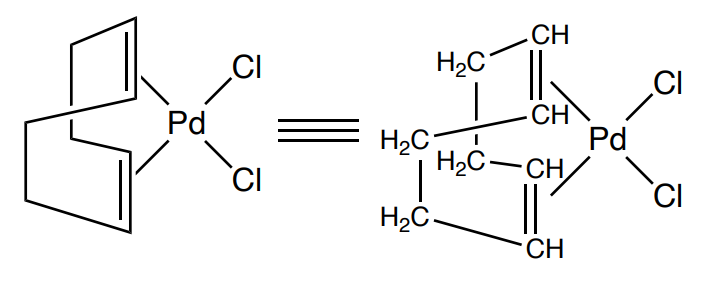
\includegraphics[width=4.8cm]{imagenes/resultados/anexo_expertos/mol3.png} & 
 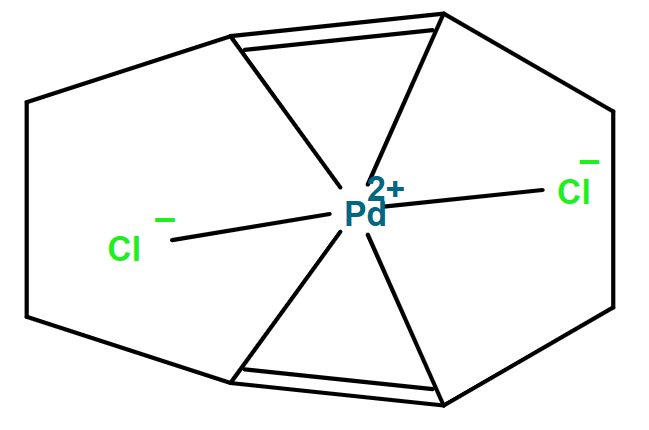
\includegraphics[width=2.6cm]{imagenes/resultados/anexo_expertos/mol3_openbabel.png} & 
 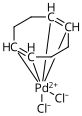
\includegraphics[width=3cm]{imagenes/sigmaAldrich/Dichloro(1,5-cyclooctadiene)palladium(II).png} & 
 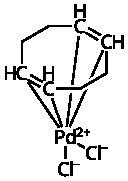
\includegraphics[width=2.2cm]{imagenes/sciFinder/pdf/Dichloro(1,5-cyclooctadiene)palladium(II).pdf} \\
\midrule

% Mol 4
 4 &
 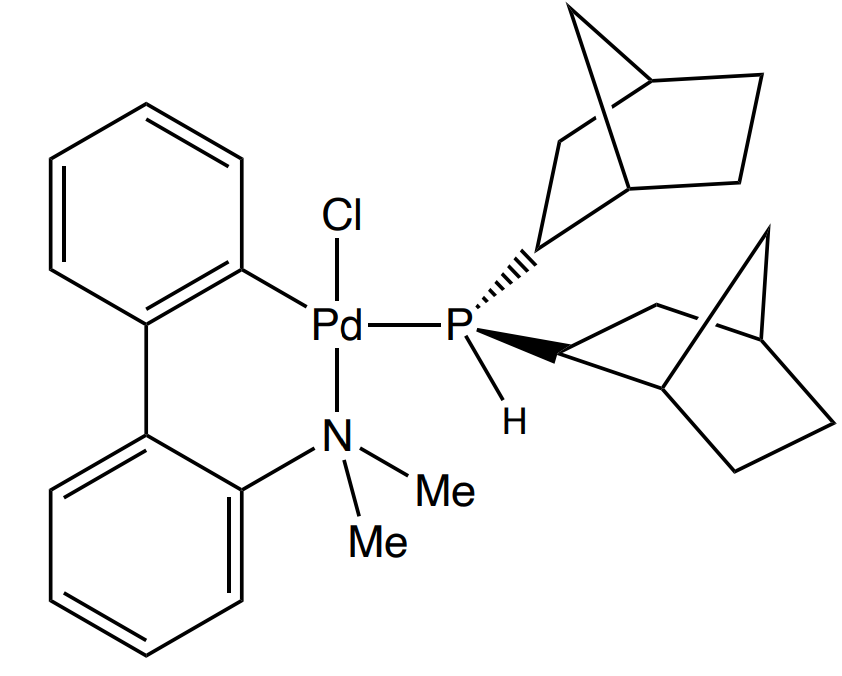
\includegraphics[width=3.5cm]{imagenes/resultados/anexo_expertos/mol4.png} & 
 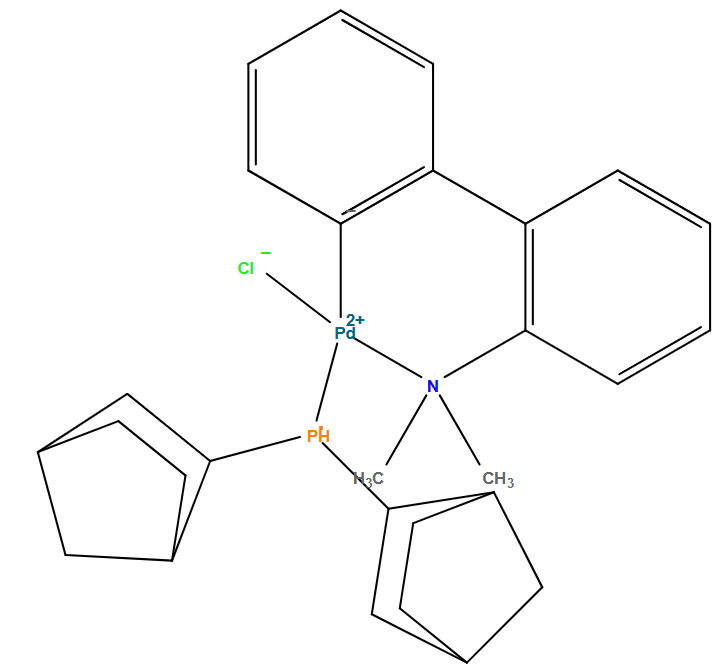
\includegraphics[width=3.5cm]{imagenes/resultados/anexo_expertos/mol4_openbabel.png} & 
 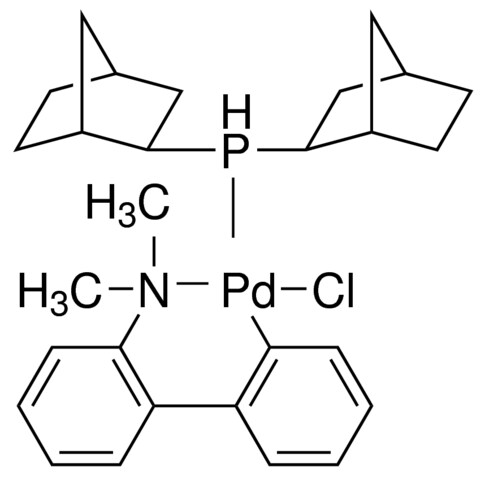
\includegraphics[width=3cm]{imagenes/sigmaAldrich/SK-CC 01A.jpeg} & 
 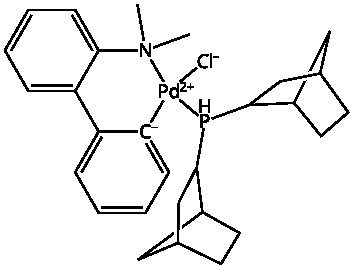
\includegraphics[width=3.3cm]{imagenes/sciFinder/pdf/SK-CC 01A.pdf} \\
\midrule

% Mol 8
 8 &
 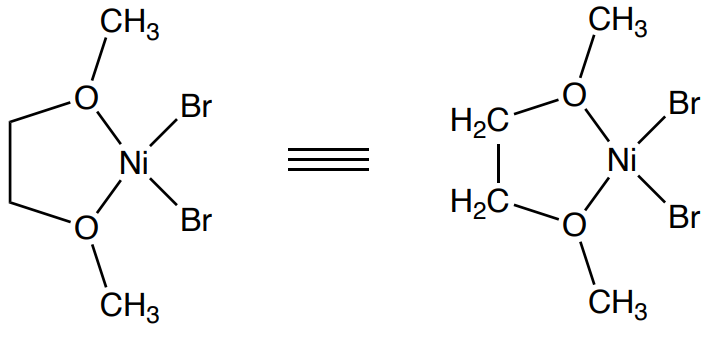
\includegraphics[width=4.7cm]{imagenes/resultados/anexo_expertos/mol8.png} & 
 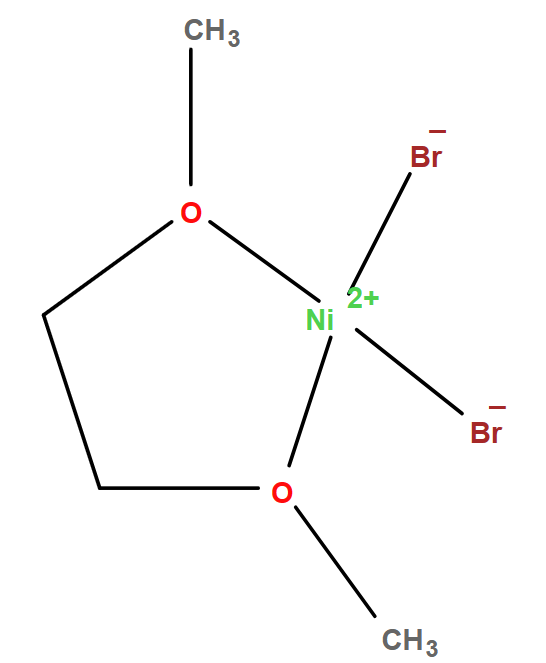
\includegraphics[width=2.2cm]{imagenes/resultados/anexo_expertos/mol8_openbabel.png} & 
 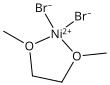
\includegraphics[width=3cm]{imagenes/sigmaAldrich/Nickel(II) bromide ethylene glycol dimethyl ether complex.png} & 
 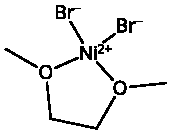
\includegraphics[width=3cm]{imagenes/sciFinder/pdf/Dibromo(1,2-dimethoxyethane)nickel(II).pdf} \\
\midrule

% Mol 9
 9 &
 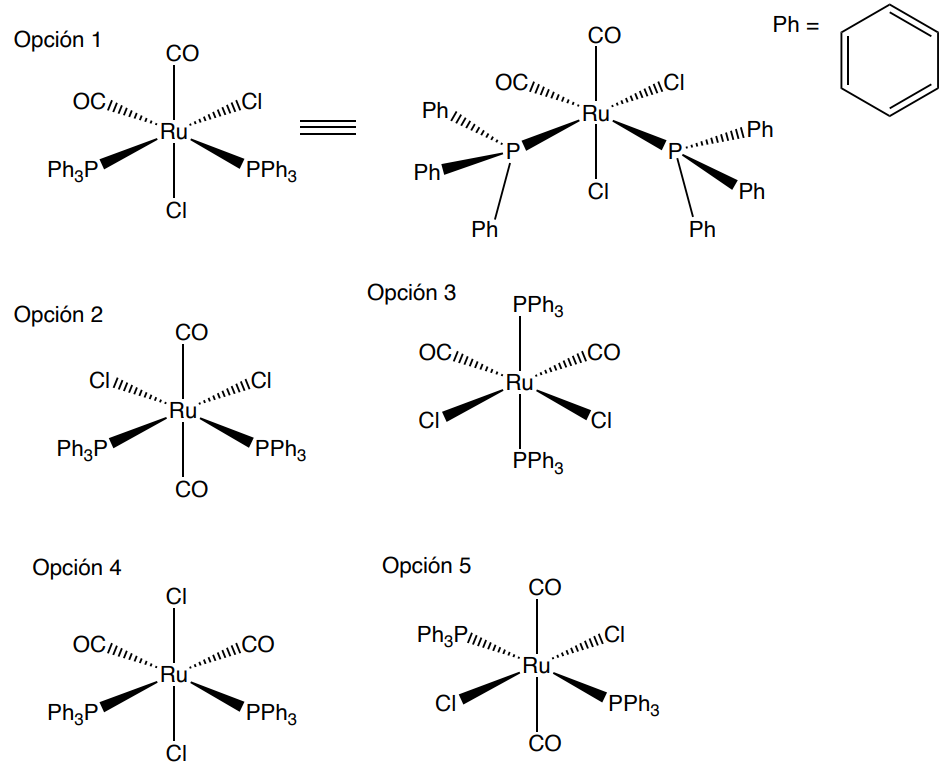
\includegraphics[width=4.2cm]{imagenes/resultados/anexo_expertos/mol9.png} & 
 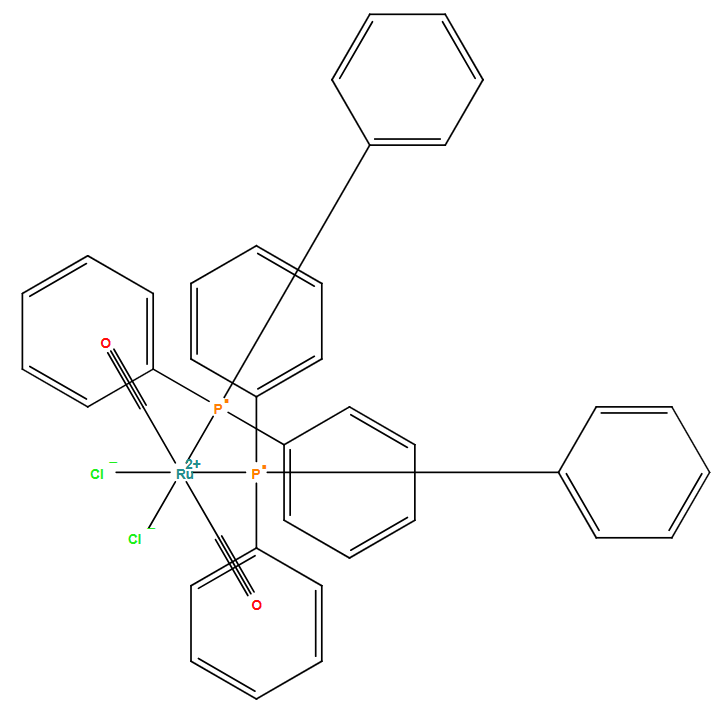
\includegraphics[width=3cm]{imagenes/resultados/anexo_expertos/mol9_openbabel.png} & 
 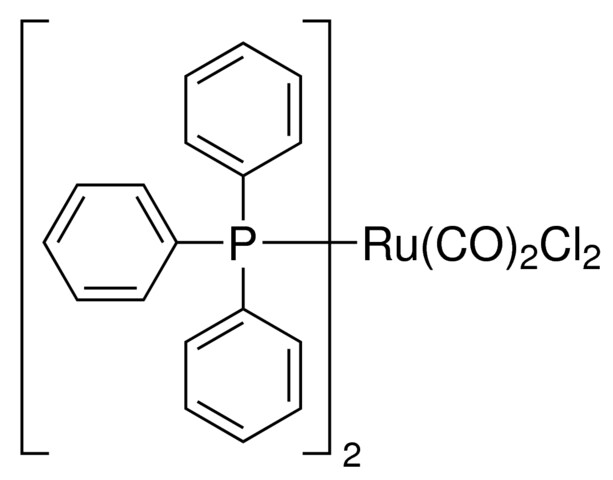
\includegraphics[width=3cm]{imagenes/sigmaAldrich/Bis(triphenylphosphine)ruthenium(II) dicarbonyl chloride.jpeg} & 
 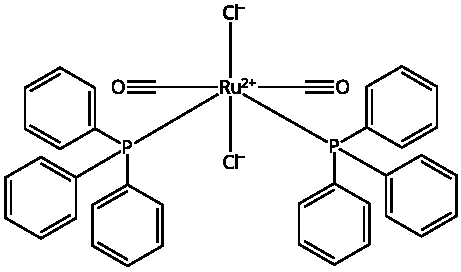
\includegraphics[width=3.4cm]{imagenes/sciFinder/pdf/Bis(triphenylphosphine)ruthenium(II) dicarbonyl chloride.pdf} \\
\midrule

% Mol 10
 10 &
 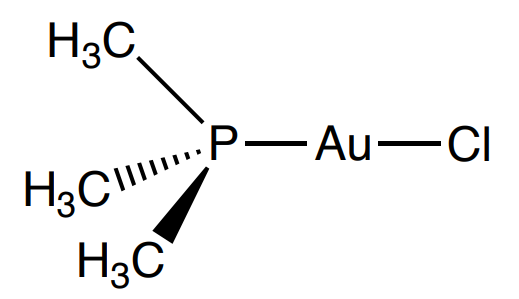
\includegraphics[width=2.7cm]{imagenes/resultados/anexo_expertos/mol10.png} & 
 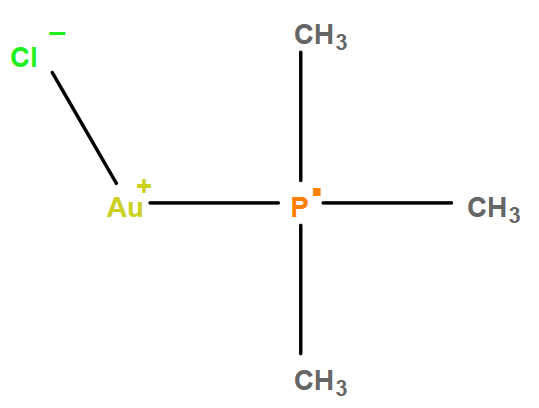
\includegraphics[width=2.7cm]{imagenes/resultados/anexo_expertos/mol10_openbabel.png} & 
 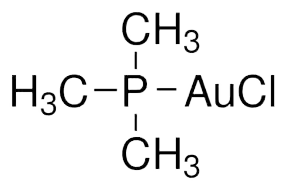
\includegraphics[width=2.5cm]{imagenes/sigmaAldrich/Chloro(trimethylphosphine)gold(I).png} & 
 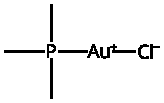
\includegraphics[width=2.5cm]{imagenes/sciFinder/pdf/Chloro(trimethylphosphine)gold(I).pdf} \\
\midrule


% Mol 25
 25 &
 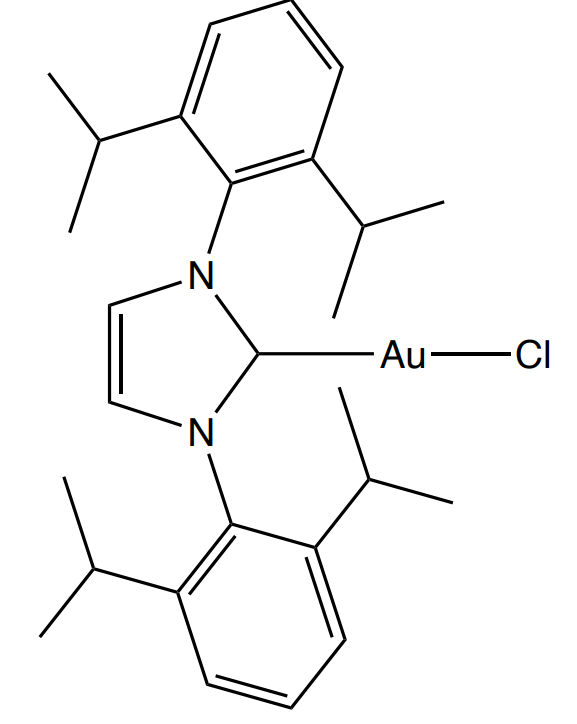
\includegraphics[width=2.2cm]{imagenes/resultados/anexo_expertos/mol25.png} & 
 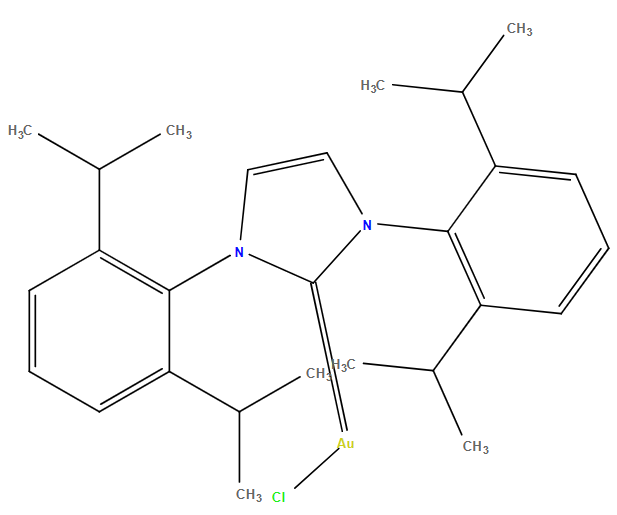
\includegraphics[width=3cm]{imagenes/resultados/anexo_expertos/mol25_openbabel.png} & 
 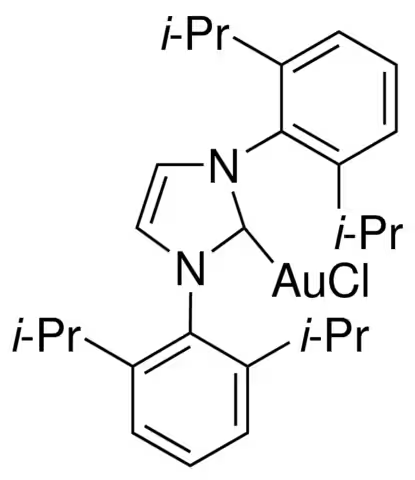
\includegraphics[width=2.2cm]{imagenes/sigmaAldrich/[(IPr)AuCl].png} & 
 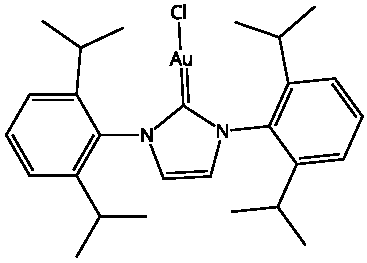
\includegraphics[width=3cm]{imagenes/sciFinder/pdf/[(IPr)AuCl].pdf} \\
\midrule


% Mol 28
 28 &
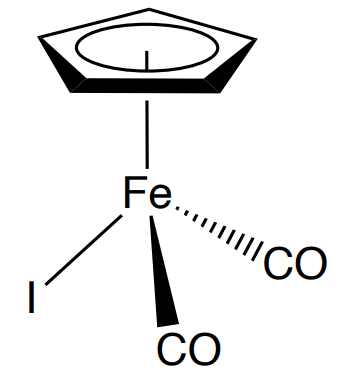
\includegraphics[width=2.2cm]{imagenes/resultados/anexo_expertos/mol28.png} & 
 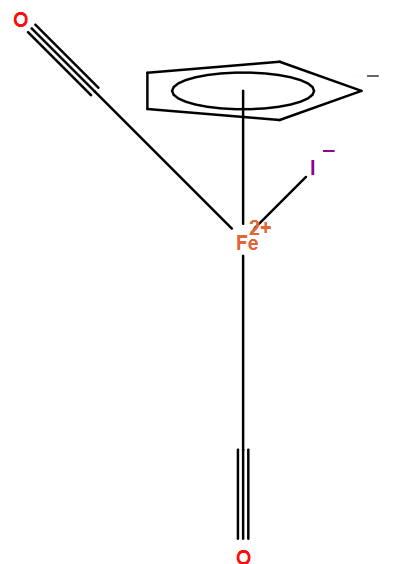
\includegraphics[width=2.2cm]{imagenes/resultados/moleculas/iron(II).png} & 
 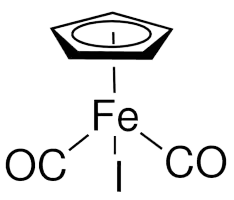
\includegraphics[width=2.2cm]{imagenes/sigmaAldrich/Dicarbonylcyclopentadienyliodoiron(II).png} & 
 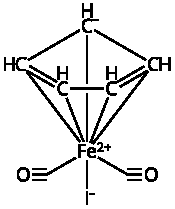
\includegraphics[width=2.2cm]{imagenes/sciFinder/pdf/Dicarbonylcyclopentadienyliodoiron(II).pdf}
% \midrule


\label{tab:expertos_dibujos}

\end{longtable}

\end{landscape}


